\section{Résultats et Discussions}

\subsection{Évaluation de l'impact de la NAO sur l'upwelling}
\subsubsection{Analyse Statistique}
\subsubsection*{Analyse générale}
Une analyse globale sur l’ensemble du territoire marocain montre que l’upwelling est principalement localisé dans la zone sud, en particulier le long de la côte atlantique sud. Cependant, il est crucial d'examiner le phénomène à l'échelle nationale pour détecter un éventuel impact des changements climatiques sur cette dynamique, notamment dans les zones traditionnellement moins affectées par l'upwelling.

\begin{figure}[H]
\centering
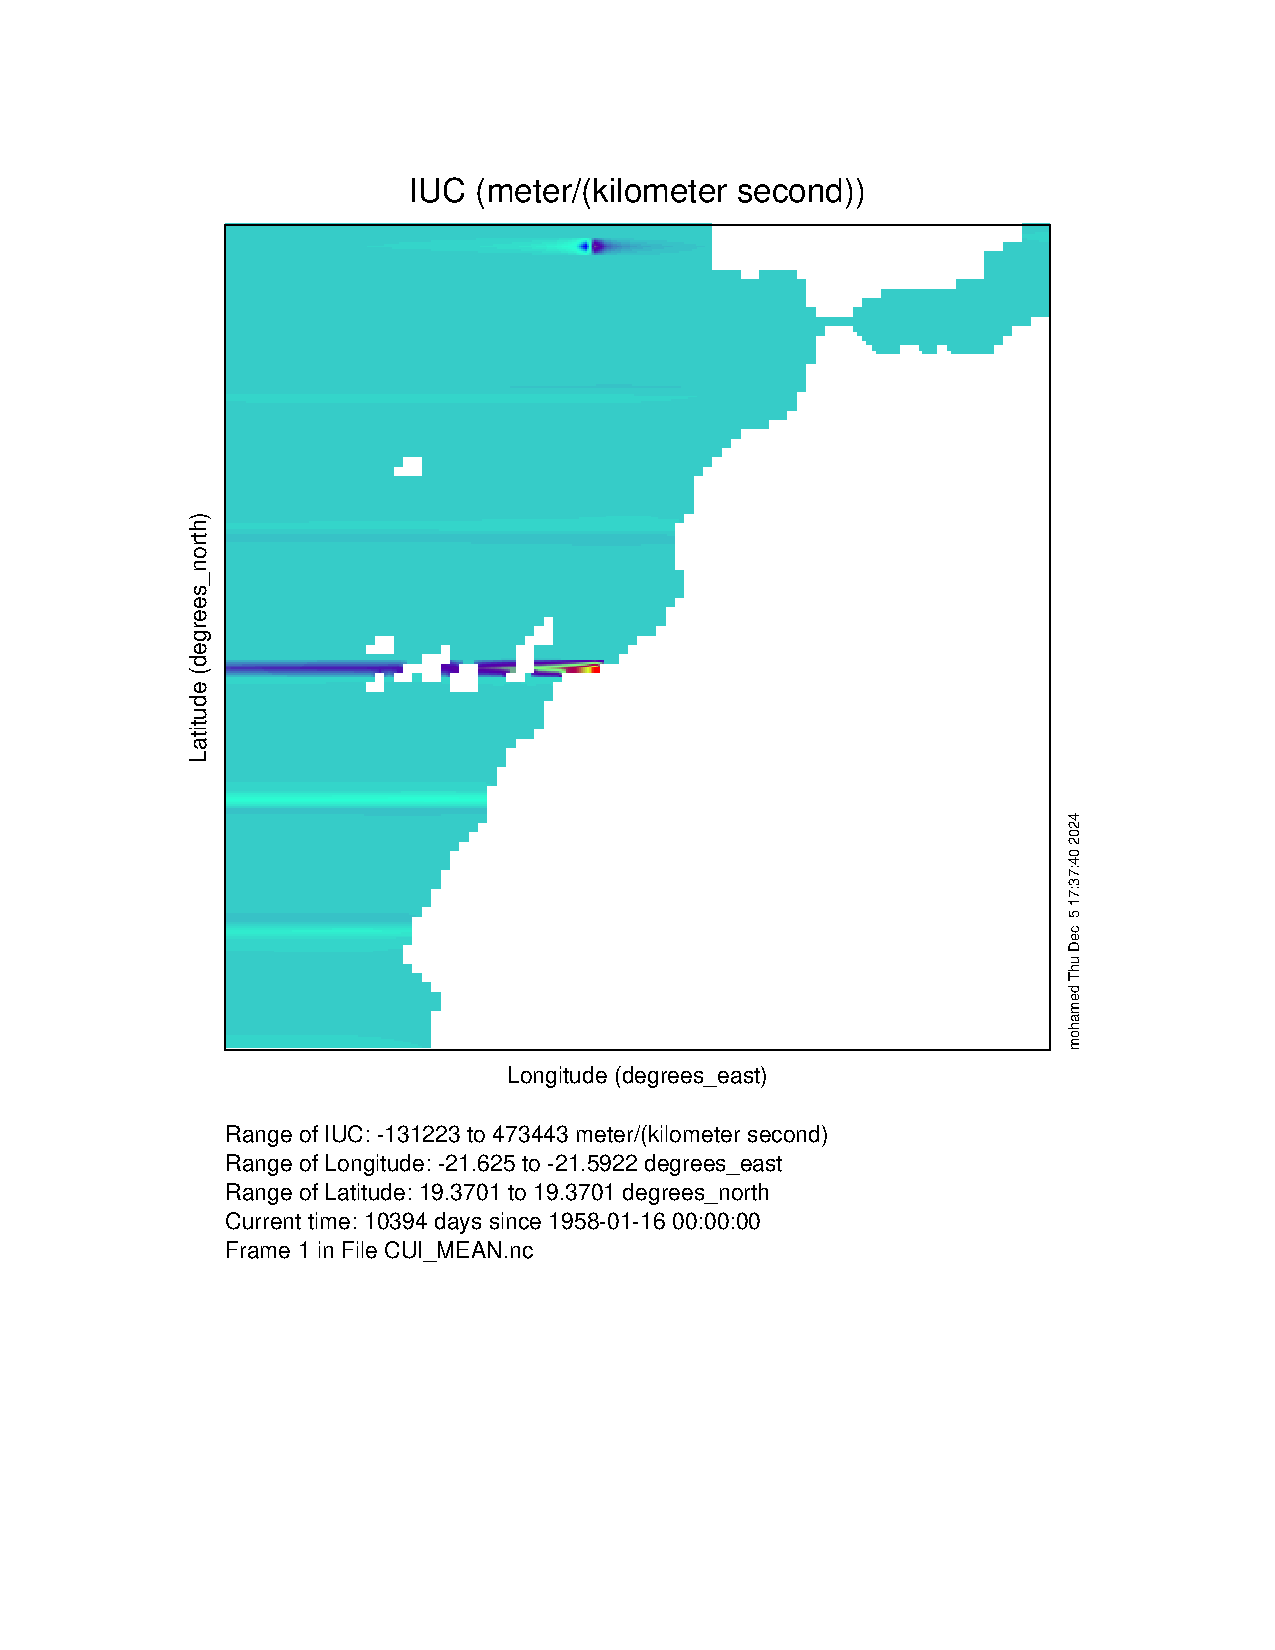
\includegraphics[scale=0.5]{ncview_output.pdf}
\caption{Climatologie de l'upwelling au Maroc (1958–2014).}
\label{fig:climatologie_upwelling}
\end{figure}

La figure~\ref{fig:climatologie_upwelling} montre la répartition spatio-temporelle de l'upwelling au Maroc, confirmant une activité accrue dans la région sud. Ces observations soulignent la nécessité de comprendre les interactions entre les indices climatiques tels que la NAO et les processus océaniques locaux.

\subsubsection*{Analyse des distributions}

La figure~\ref{fig:distributions} illustre les distributions de probabilité de l’indice d'upwelling côtier (CUI) et de l'oscillation nord-atlantique (NAO). 

\begin{figure}[H]
\centering
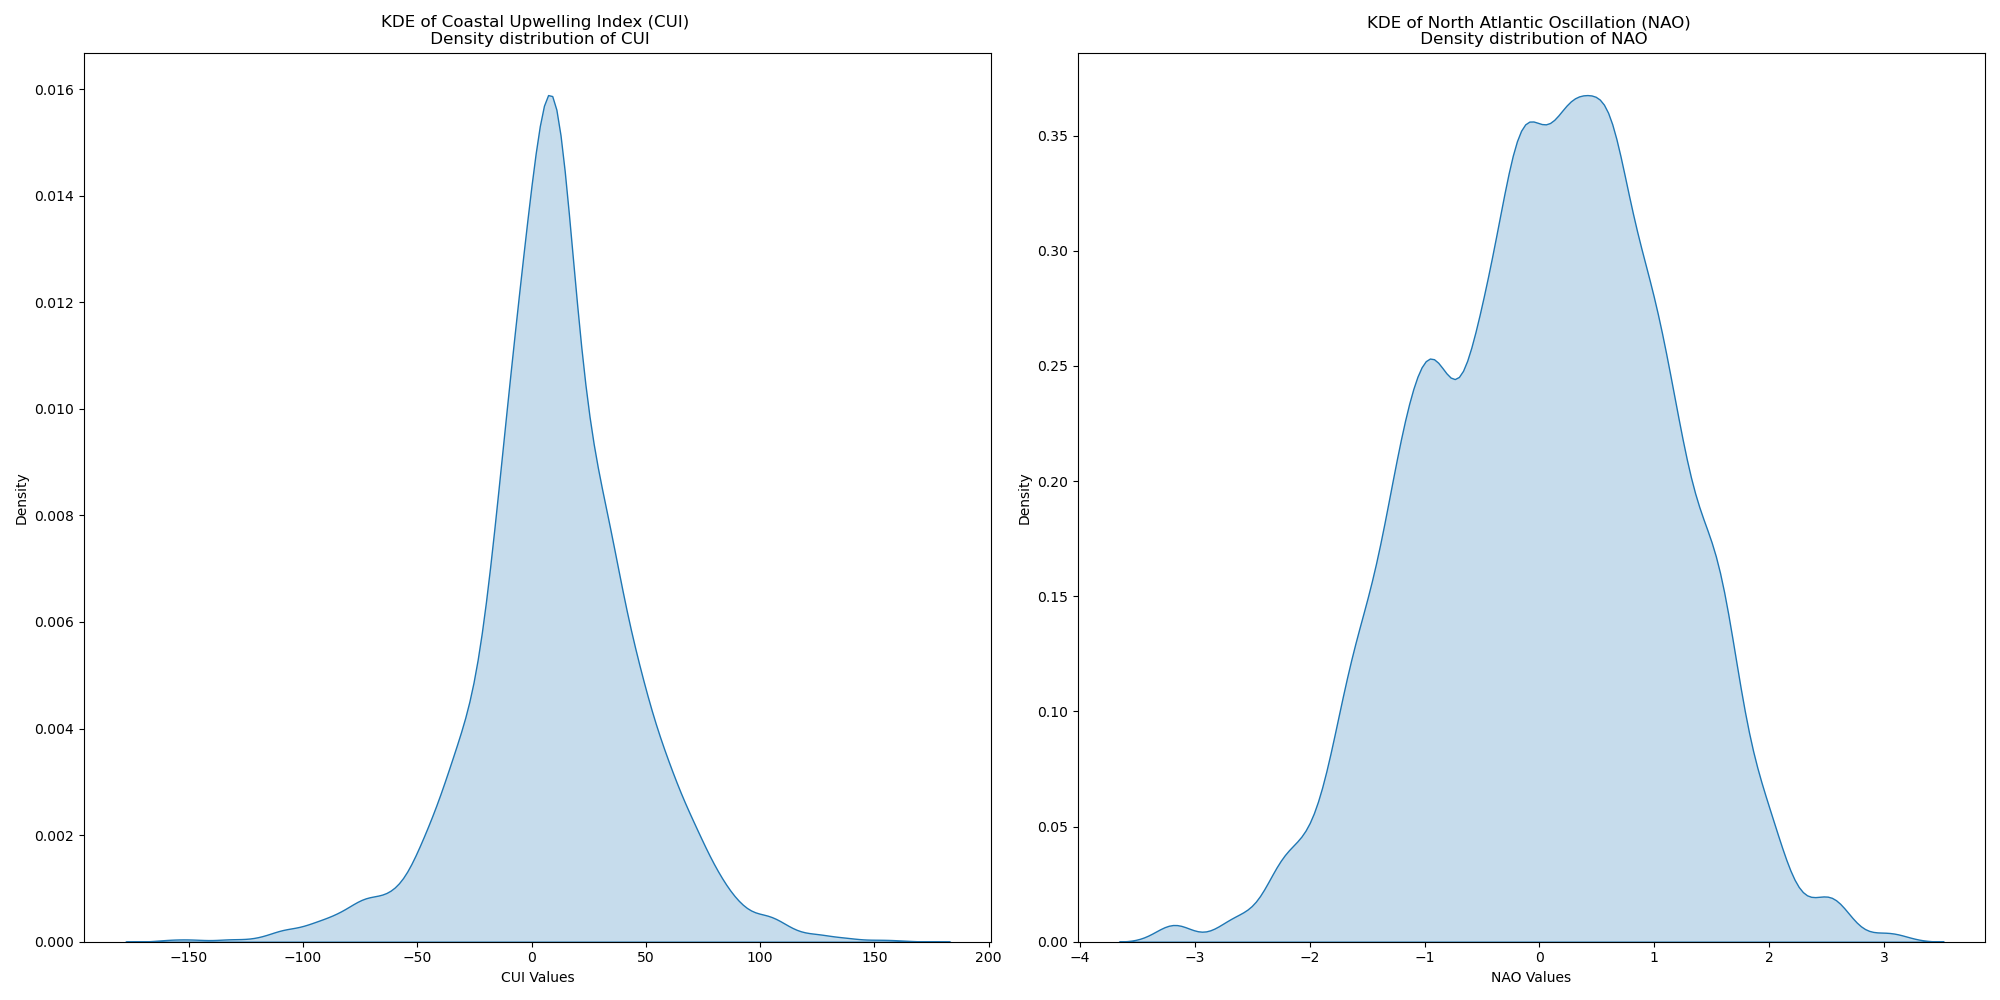
\includegraphics[scale=0.3]{kde_nao_cui.png}
\caption{Distribution de probabilité pour NAO et CUI.}
\label{fig:distributions}
\end{figure}

Les deux indices suivent une distribution normale centrée autour de zéro. Cette symétrie indique que les valeurs extrêmes (positives ou négatives) sont rares, tandis que la majorité des données se concentre autour de la moyenne. Cette caractéristique statistique suggère des variations régulières, bien adaptées pour des analyses de corrélation.

\subsubsection*{Analyse de la corrélation NAO-CUI}
\begin{figure}[H]
\centering
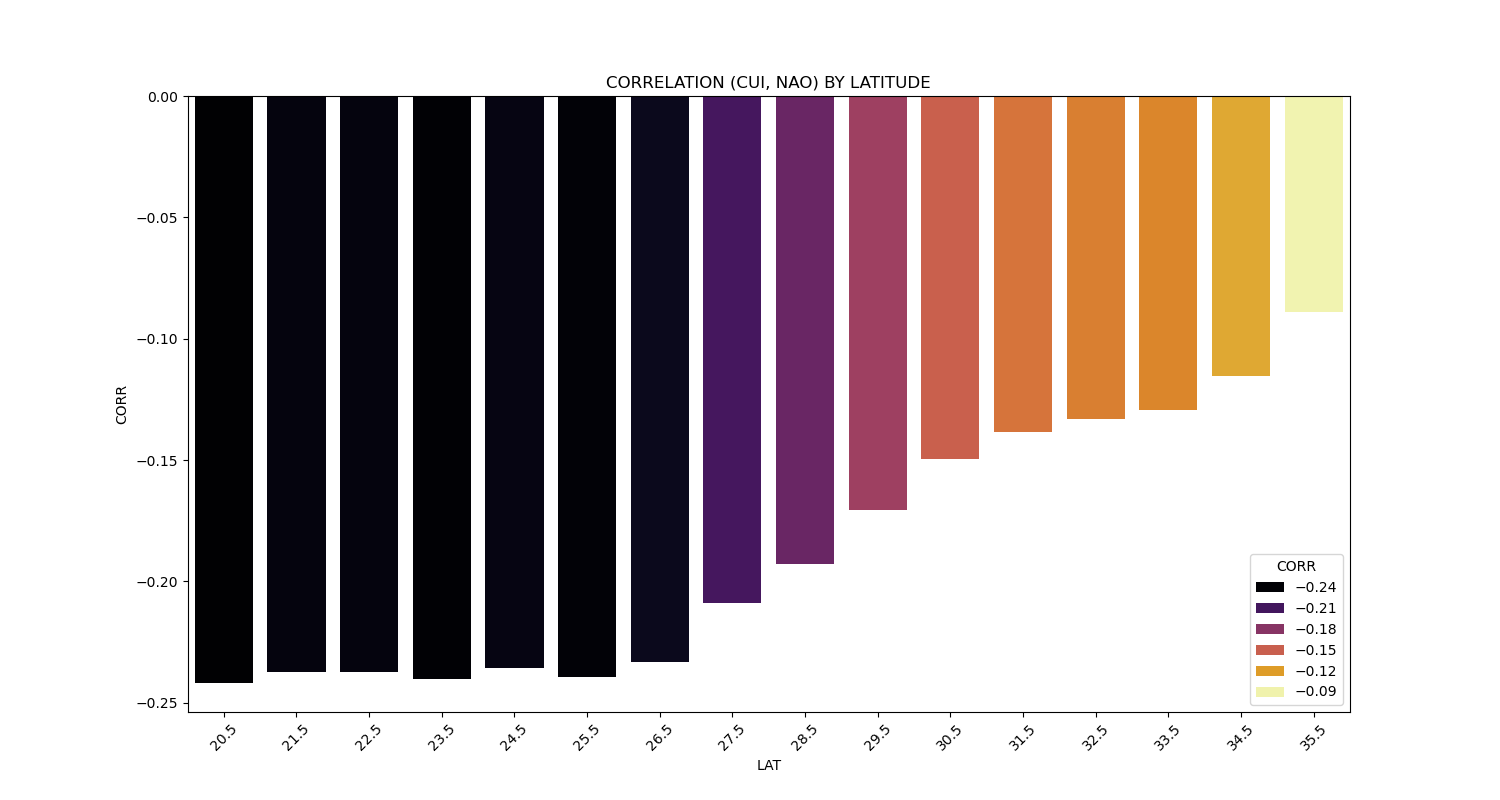
\includegraphics[scale=0.3]{corr.png}
\caption{Corrélation entre la NAO et le CUI en fonction de la latitude.}
\label{fig:correlation}
\end{figure}

La figure~\ref{fig:correlation} met en évidence une corrélation négative entre la NAO et le CUI, avec une intensité qui varie selon la latitude. Les observations principales incluent :
\begin{itemize}
    \item \textbf{20.5 - 26.5 :} La corrélation est fortement négative, indiquant un impact marqué de la NAO sur l'upwelling. Cela correspond aux régions où l’upwelling est historiquement le plus actif, notamment entre Agadir et Lagouira.
    \item \textbf{27.5-35.5:} La corrélation diminue en intensité, devenant presque nulle. Cela reflète un moindre impact de la NAO sur l’upwelling dans ces régions.
\end{itemize}

Ces résultats corroborent les observations sur le terrain, où les zones sud du Maroc présentent une productivité biologique élevée, stimulée par l'upwelling, ce qui favorise des activités de pêche dynamiques.

\subsubsection{Impact de la phase de la NAO sur l'upwelling}
Pour explorer davantage l’effet de la NAO, l’analyse a été subdivisée en deux phases distinctes : la phase positive (NAO+) et la phase négative (NAO-). La figure~\ref{fig:impact_phases} illustre les variations du CUI pour chaque phase. L'analyse du graphe montre que l'intensité de l'upwelling est plus élevée pendant les phases de NAO négative (NAO-) par rapport aux phases de NAO positive (NAO+). Cela reflète que les conditions océaniques et les régimes de vent pendant les phases de NAO- favorisent une augmentation de l'upwelling, tandis que les phases de NAO+ entraînent une réduction de son intensité.

\begin{figure}[H]
\centering
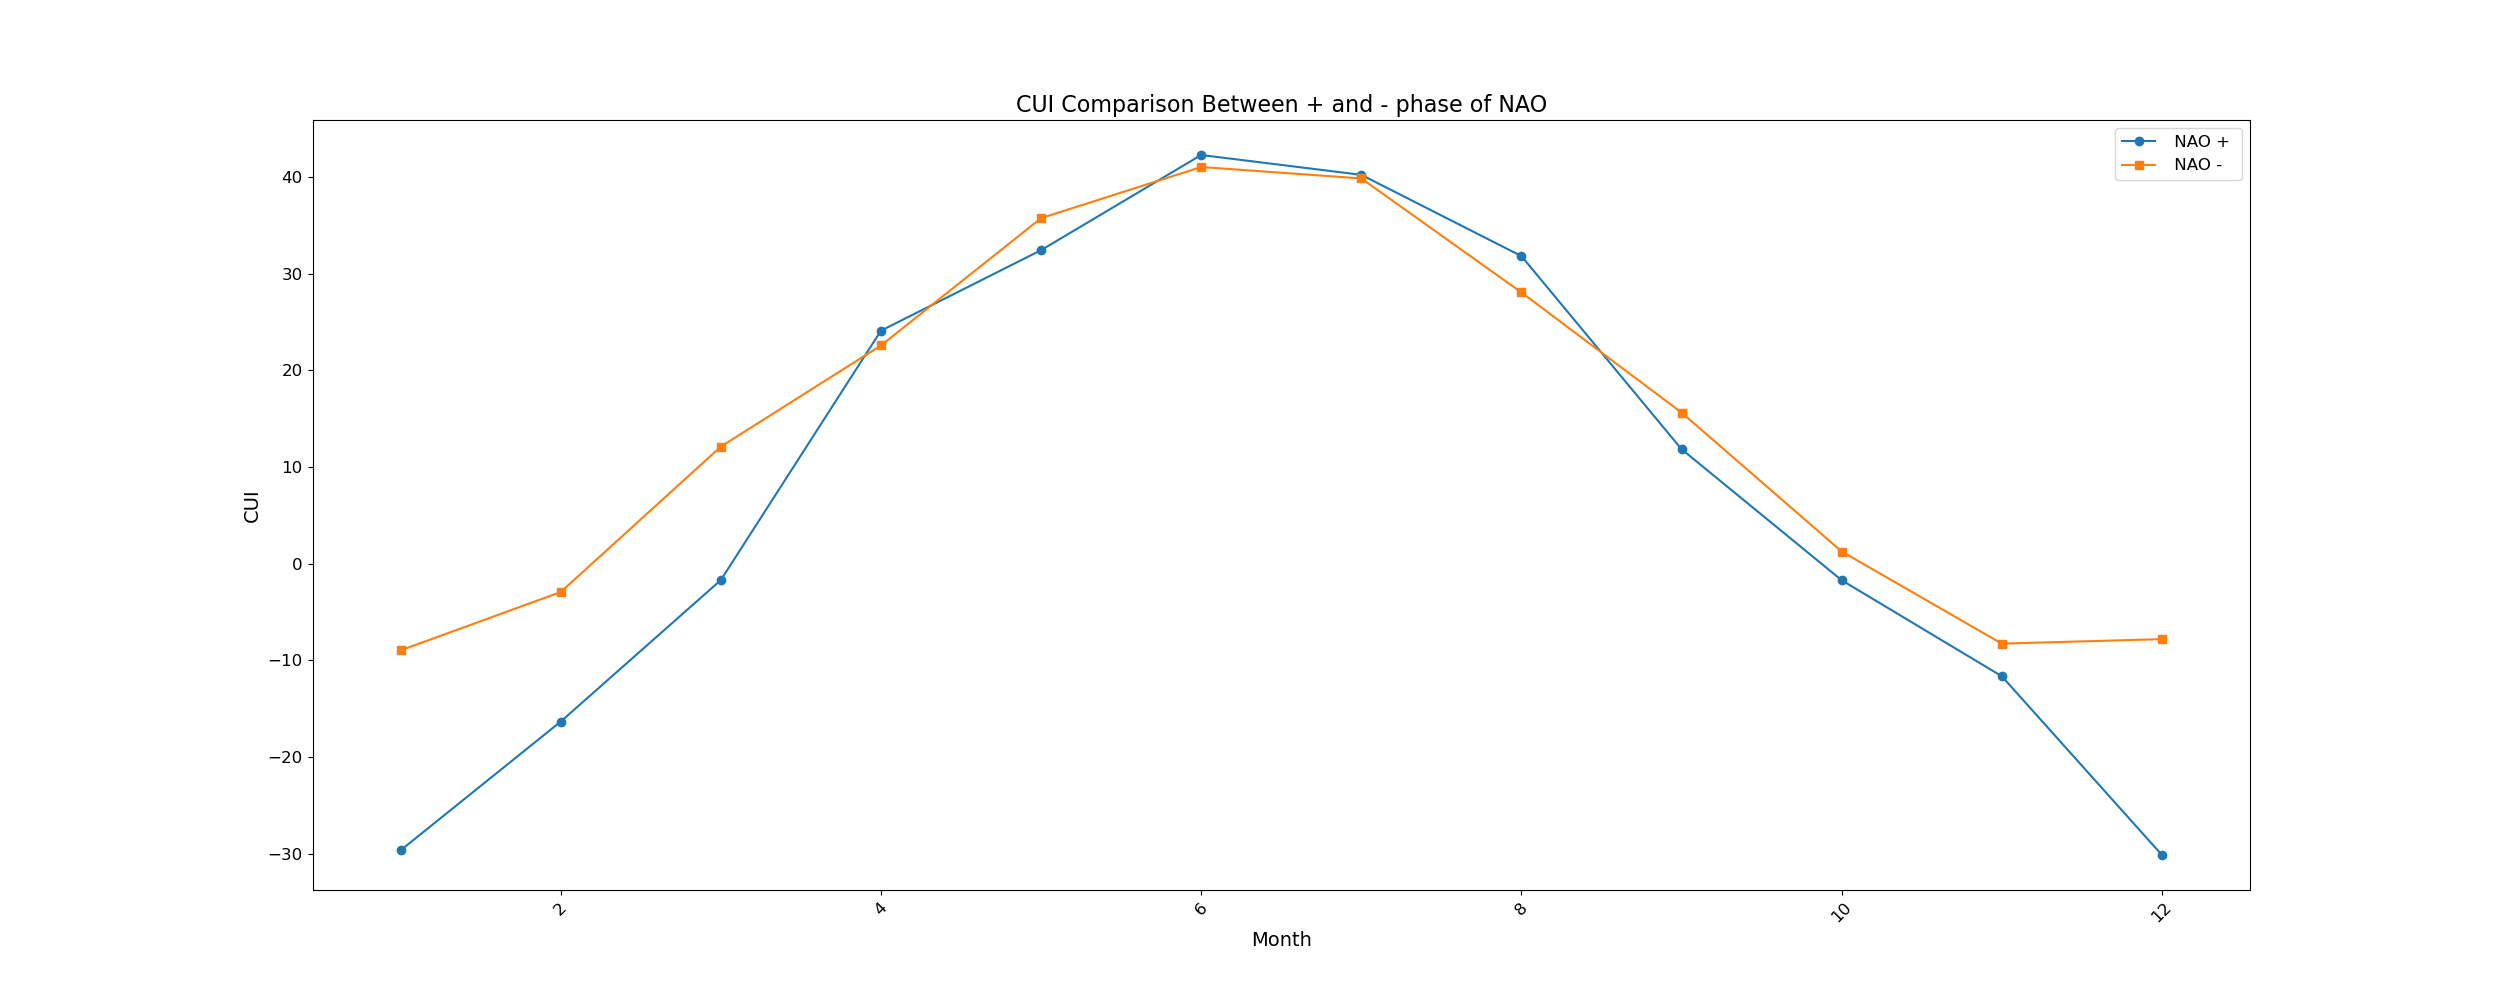
\includegraphics[scale=0.3]{CUI_NAO_PHASES.png}
\caption{Analyse de l'impact des phases de la NAO sur le CUI.}
\label{fig:impact_phases}
\end{figure}

\subsubsection*{Phase positive de la NAO (NAO+)}
\begin{figure}[H]
\centering
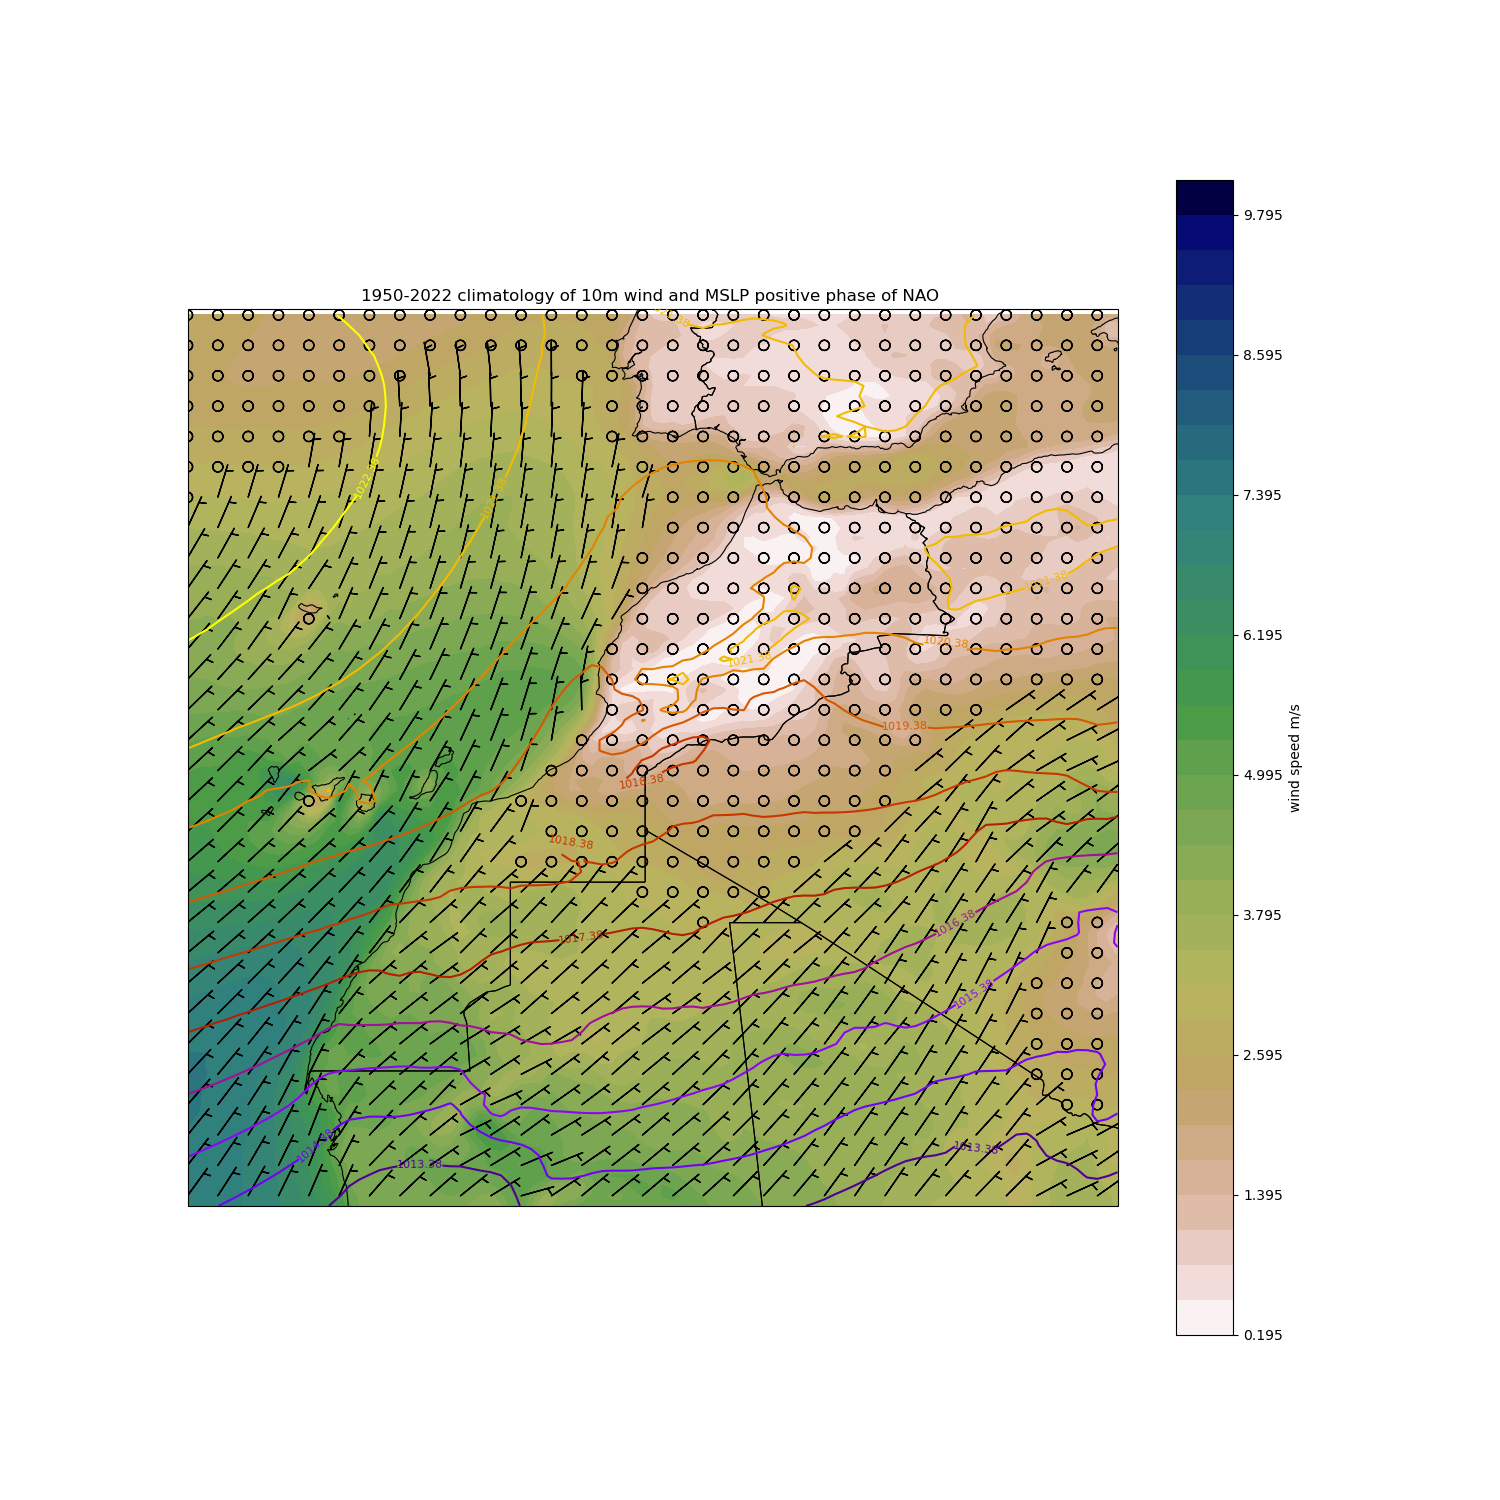
\includegraphics[scale=0.3]{POS_PHASE.png}
\caption{Climatologie du vent et de la pression pour la phase NAO+ (1950–2022).}
\label{fig:nao_positive}
\end{figure}

Lors de la phase NAO+, les caractéristiques atmosphériques et océaniques suivantes sont observées :
\begin{itemize}
    \item \textbf{Direction du vent :} Les vents soufflent moins parallèlement à la côte, réduisant l'efficacité du mécanisme d'upwelling. Cette désorientation est particulièrement visible dans les zones méridionales.
    \item \textbf{Intensité du vent :} La vitesse moyenne du vent ne dépasse pas 3 m/s (environ 6 nœuds), limitant le transport d'Ekman et la remontée des eaux froides riches en nutriments.
    \item \textbf{Impact sur le CUI :} Une phase NAO+ est associée à une diminution significative de l’intensité de l’upwelling, affectant négativement la productivité marine, en particulier dans les zones à forte dépendance économique sur la pêche.
\end{itemize}

\subsubsection*{Phase négative de la NAO (NAO-)}
\begin{figure}[H]
\centering
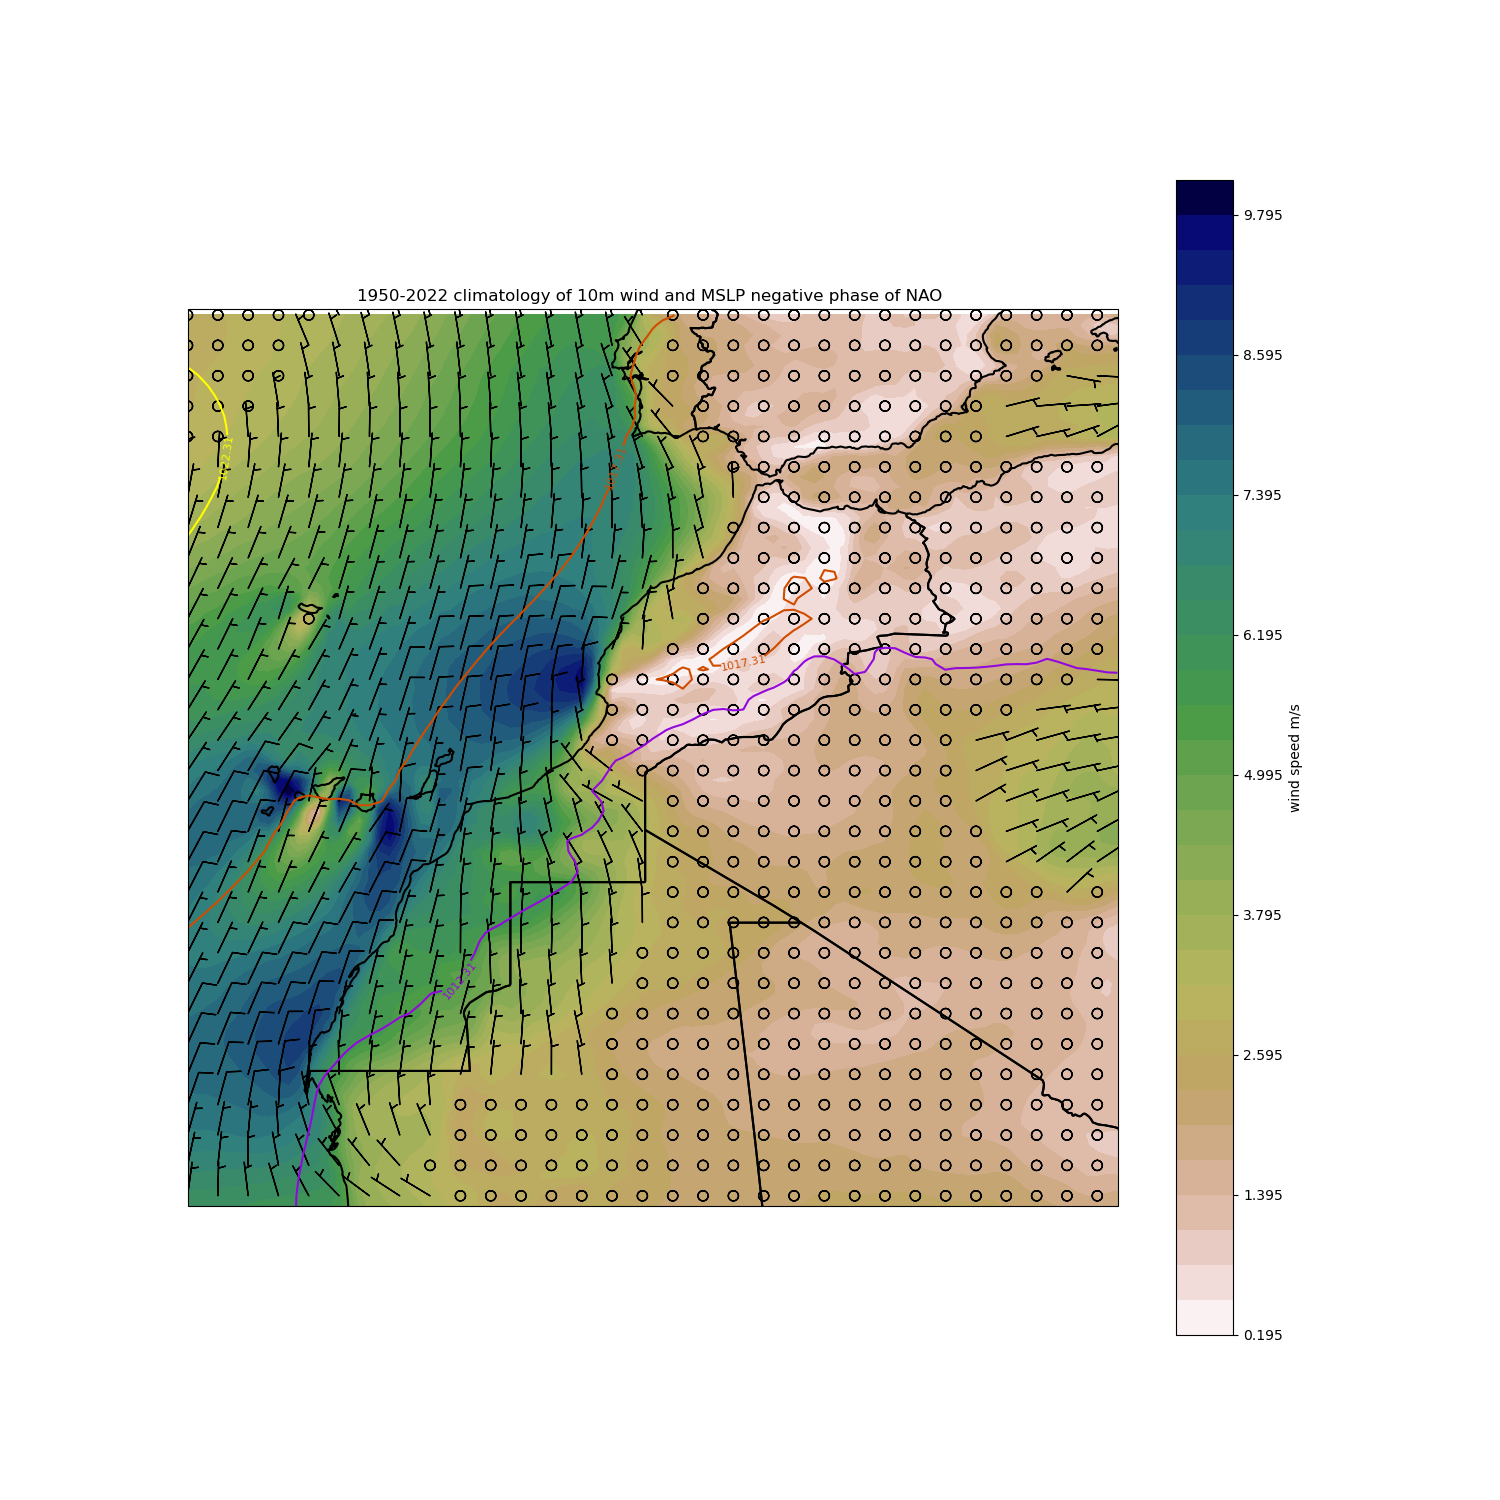
\includegraphics[scale=0.3]{NEG_PHASE.png}
\caption{Climatologie du vent et de la pression pour la phase NAO- (1950–2022).}
\label{fig:nao_negative}
\end{figure}

En revanche, la phase NAO- est caractérisée par des conditions favorables à l’upwelling :
\begin{itemize}
    \item \textbf{Direction du vent :} Les vents deviennent parallèles à la côte, favorisant un transport d'Ekman plus efficace. Cet alignement optimal est particulièrement marqué dans la région sud.
    \item \textbf{Intensité du vent :} Les vitesses moyennes atteignent environ 10 m/s, augmentant considérablement la dynamique de remontée des eaux froides.
    \item \textbf{Impact sur le CUI :} Une phase NAO- stimule fortement l’upwelling, renforçant la productivité biologique et soutenant les écosystèmes marins. Ces conditions sont idéales pour les activités de pêche dans la région.
\end{itemize}

\subsubsection{Analyse de la tendance de l'upwelling}
l'analyse de l'indice de l'upwelling côtier par latitude montre que l'upwelling concerne surtout la zone sud. l'intensité de cet indice diminue significativement avec la latitude. pour le sud du Maroc le CUI peut atteindre jusqu'à 150 m/s.Quant au nord du pays, l'intensité ne dépasse pas généralement 70m/s.

\begin{figure}[H]
\centering
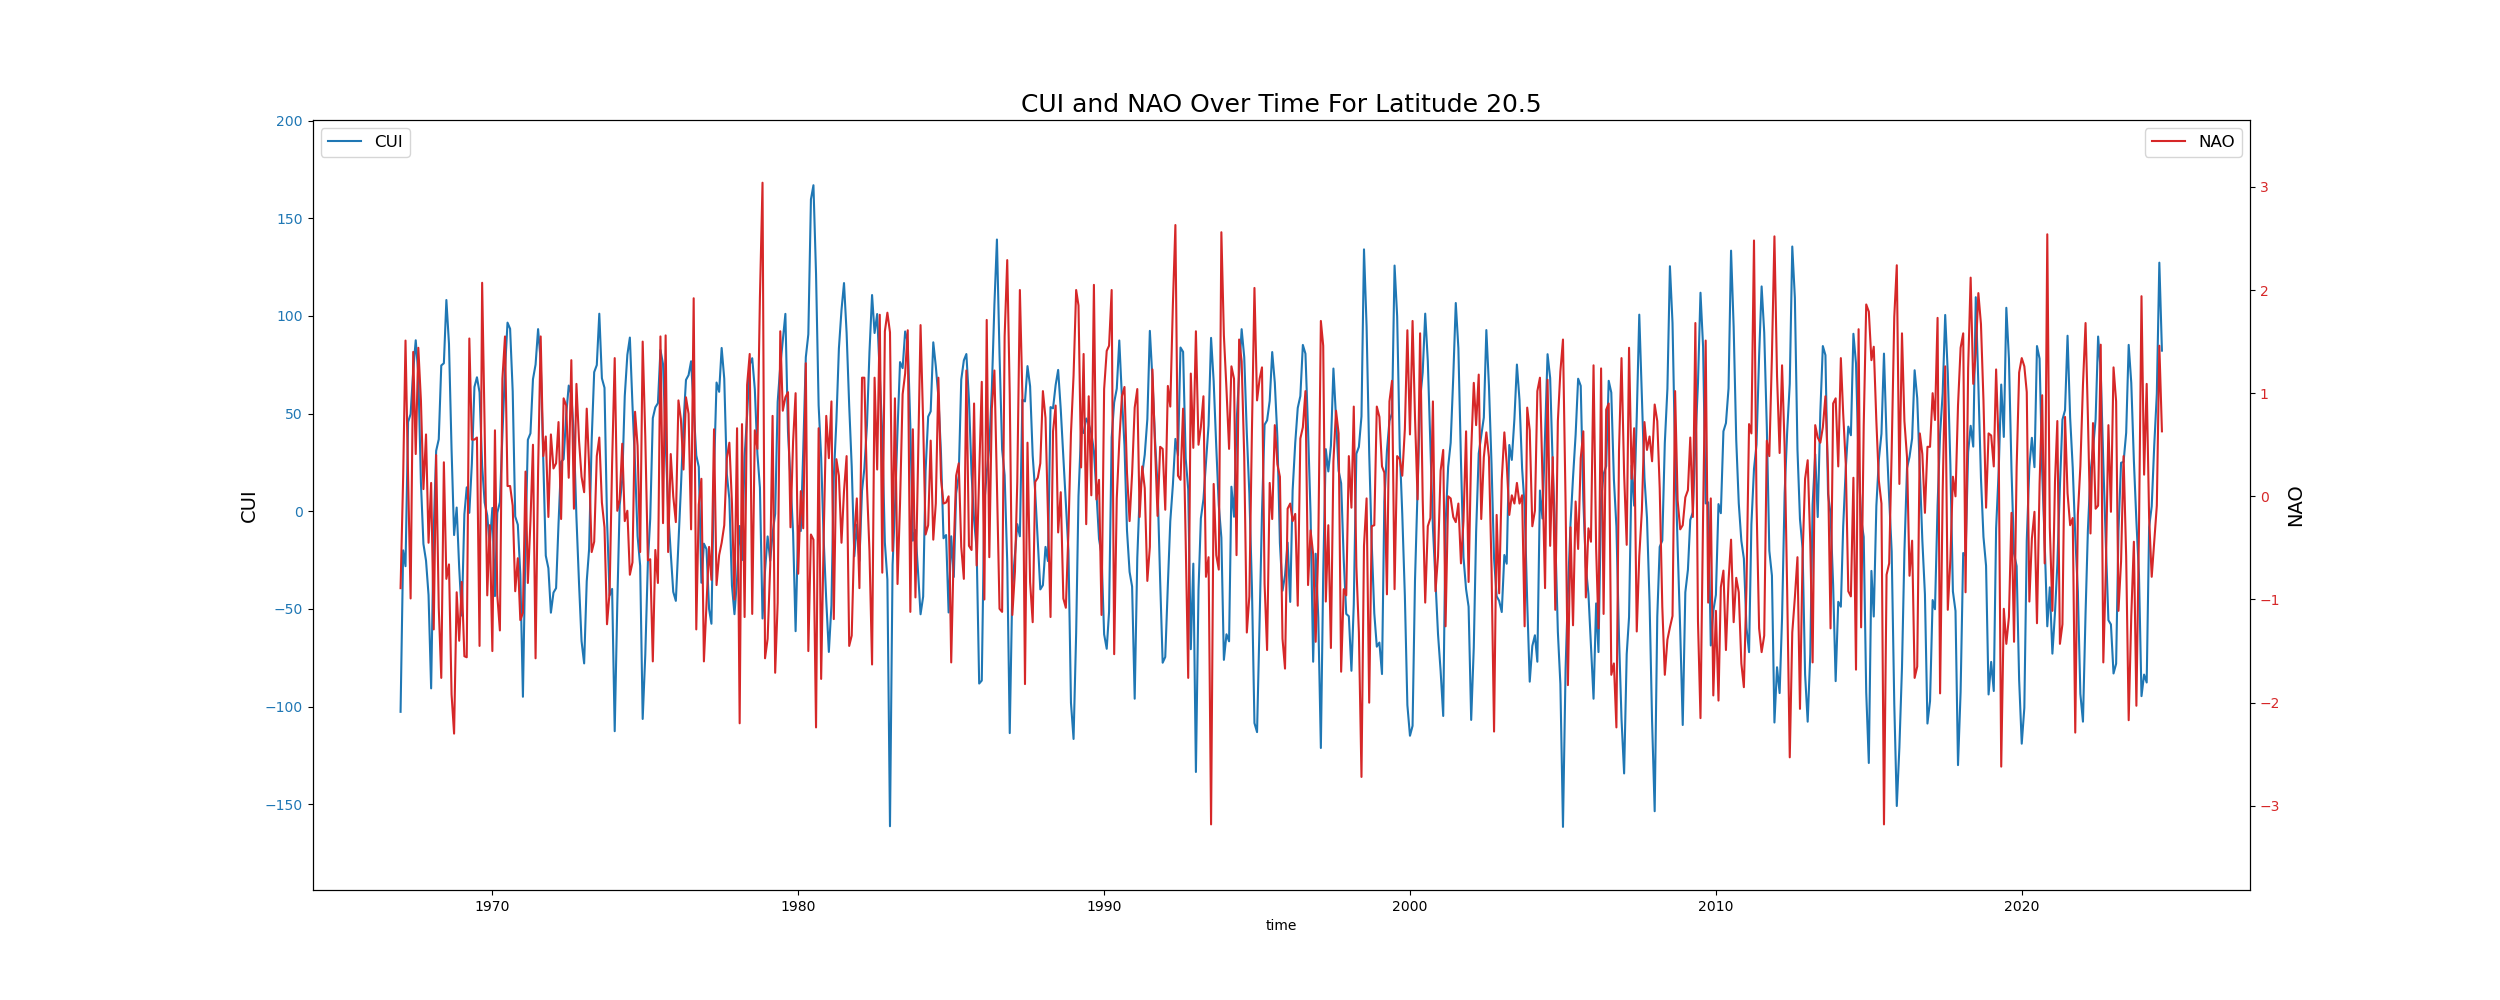
\includegraphics[scale=0.2]{CUI_NAO_20.5.png}
\caption{le CUI-NAO pour la latitude 20.5 1967-2022}
\end{figure}


\begin{figure}[H]
\centering
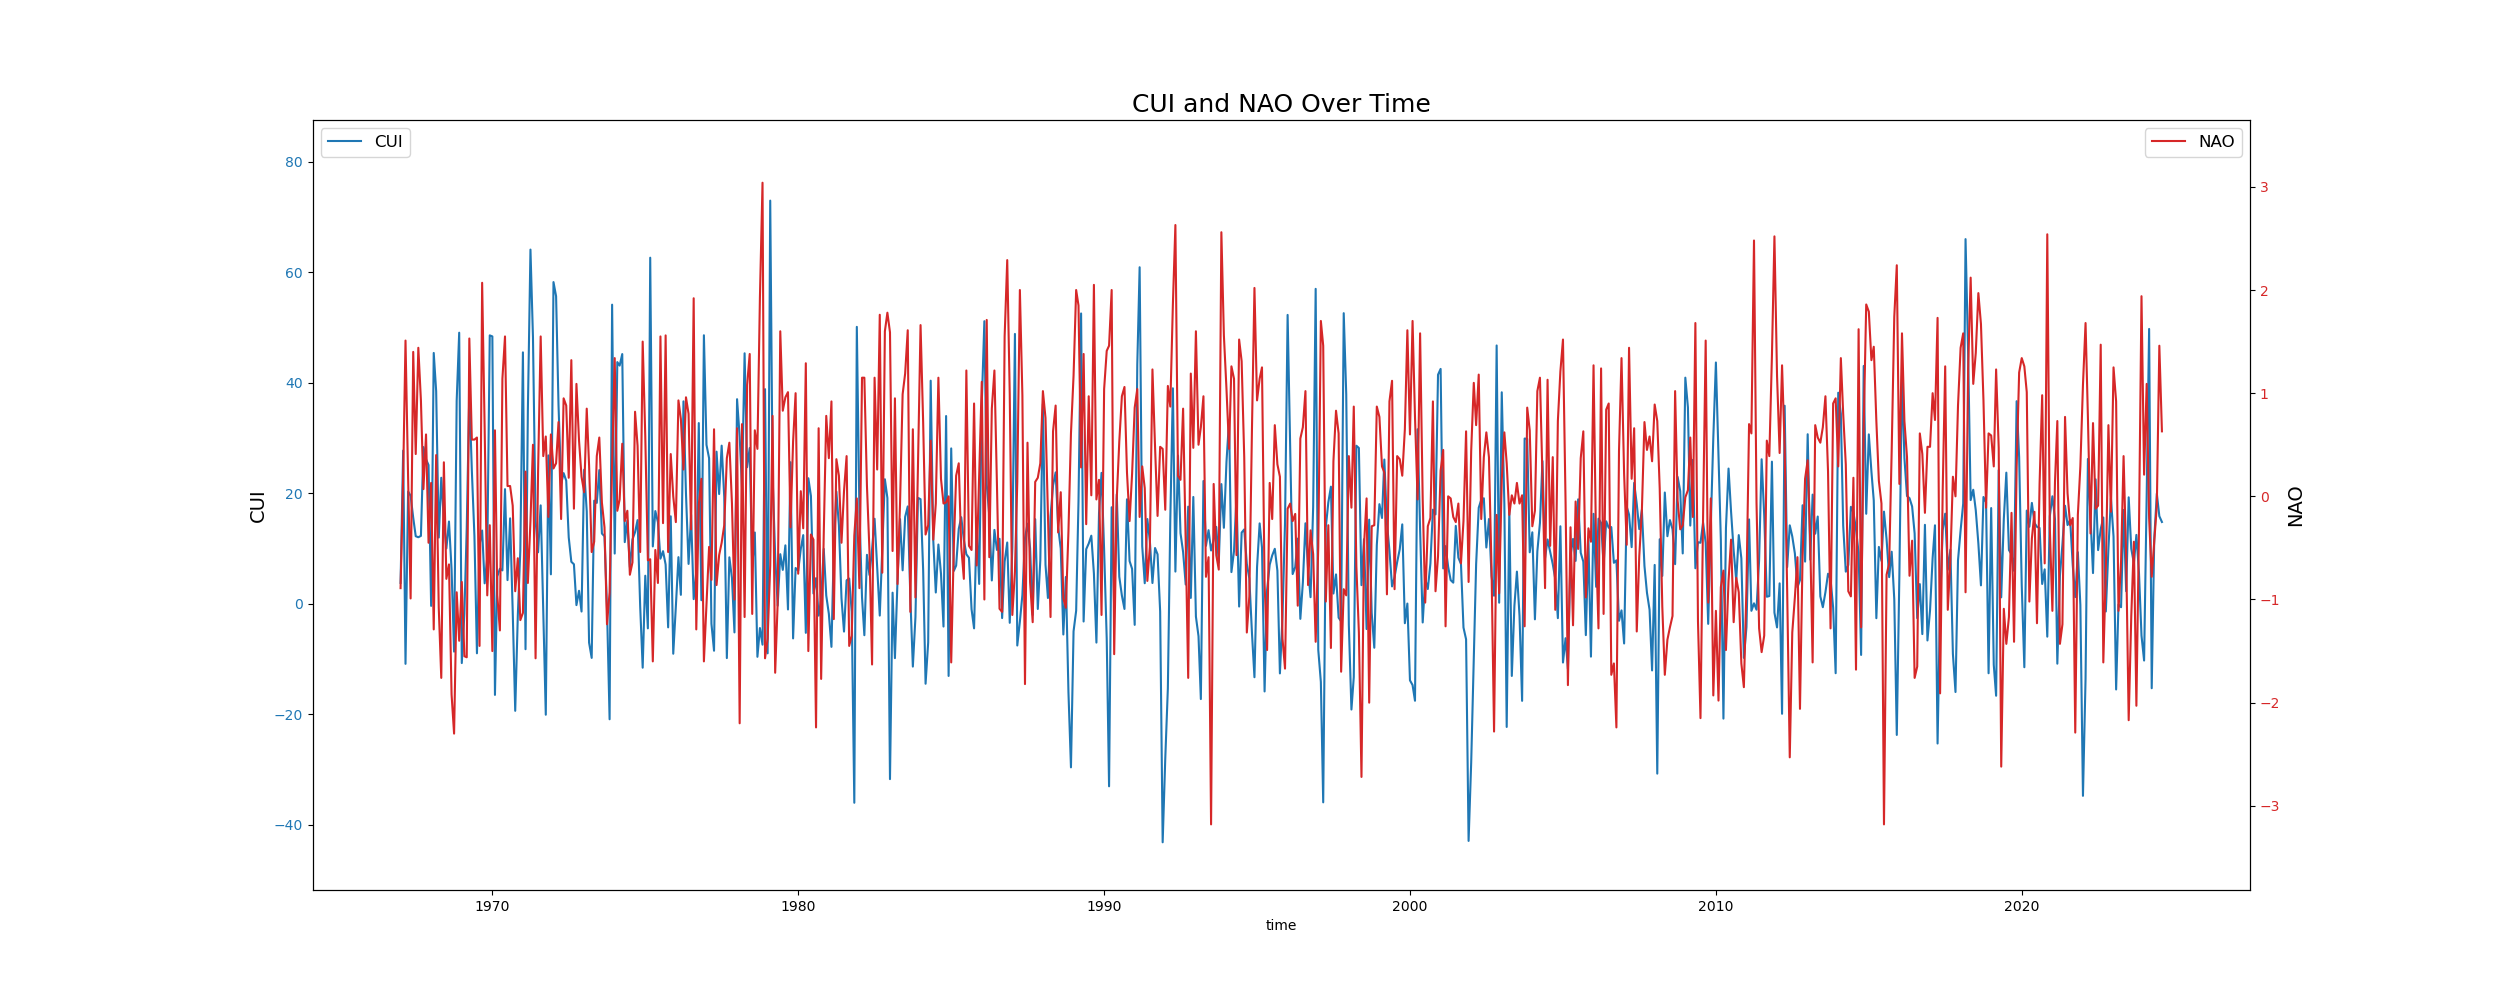
\includegraphics[scale=0.2]{CUI_NAO_34.5.png}
\caption{le CUI-NAO pour la latitude 34.5 1967-2022}
\end{figure}

Le CUI montre une grande variabilité d'une année à l'autre, avec des valeurs allant de + - 150 dans le sud du Maroc et +- 50 dans le Nord du Pays . Cette variabilité reflète la dynamique complexe des événements d'upwelling le long de la côte atlantique du Maroc dans le Sud. Le NAO, en revanche, montre également une grande variabilité temporelle avec des phases positives et négatives marquées. \\
\vspace{0.5cm}

\textbf{\textit{Relations entre le CUI et le NAO}}
L’analyse visuelle du graphique révèle une relation inversée entre le CUI et le NAO. Lorsque le NAO est en phase positive, le CUI tend à diminuer, et inversement lorsque le NAO est en phase négative, le CUI augmente. Cette relation s’explique par la direction et l’intensité des vents dominants sur l’Atlantique Nord. En phase négative du NAO, les vents deviennent plus variés et souvent plus faibles, mais la configuration sur le Maroc est caractérisé par un vent plus fort surtout dans le sud avec une direction parfaitement paralléle à la cote favorisant ainsi un CUI plus élevé. 

\textbf{\textit{Impact du changement climatique}}
Sur la longue période couverte par le graphique (1967-2022), bien que l'on observe des fluctuations importantes dans le Coastal Upwelling Index (CUI), il n'y a pas de tendance claire de baisse généralisée. Le CUI montre des variations substantielles d’une décennie à l’autre, sans indication évidente d’une diminution continue à travers la période observée. Cela pourrait suggérer que les effets du changement climatique sur le régime des vents et les températures de surface de la mer n'ont pas encore entraîné une réduction systématique de l’upwelling le long de la côte atlantique marocaine.

Les phases de la North Atlantic Oscillation (NAO) montrent également une certaine variabilité, avec des périodes de hausse et de baisse qui ne correspondent pas systématiquement à une tendance de long terme vers la diminution du CUI. Cela indique que les régimes climatiques naturels continuent d'influencer les processus océaniques, en maintenant la complexité des interactions entre le climat et les écosystèmes marins.

Ainsi, malgré les préoccupations liées aux effets du changement climatique, les données actuelles ne permettent pas d’établir une tendance significative vers la baisse du CUI. Il est nécessaire de continuer à surveiller attentivement ces paramètres et d’approfondir les analyses pour mieux comprendre les impacts réels du changement climatique sur les régimes d’upwelling en Atlantique.
